\chapter{Implementation \& Architecture}

This chapter details the engineering and algorithmic depth built during the development of MERIT. It explicitly breaks down the implementation of the system's three core pillars: Multi-Source Fusion, Explainability, and Extensibility. 
The discussion moves from the high-level system architecture to the specific mathematical models and software engineering optimisations that define the MERIT pipeline.

\definecolor{ImperialBlue}{RGB}{0, 0, 255}    % Imperial Blue
\definecolor{ProcessBlue}{RGB}{0, 145, 212}   % Process Blue for contrast
\definecolor{LightBlue}{RGB}{235, 245, 255}   % Adjusted background blue
\definecolor{CoolGrey}{RGB}{158, 161, 162}    % Neutral Grey

\section{Implementation \& Architecture}


\subsection{High-Level System Design}
MERIT is partitioned into three distinct functional domains: 
\textbf{Extraction}, \textbf{Configuration}, and \textbf{Execution}. 
Figure \ref{fig:high_level_arch} illustrates the orchestration between these layers.

% Figure 4.1: High-Level System Design
\begin{figure}[htbp]
    \centering
    \begin{tikzpicture}[
        node distance=1.2cm and 1.8cm,
        arch_domain/.style={draw=ImperialBlue, fill=LightBlue!30, dashed, rounded corners, thick, inner sep=15pt},
        arch_logic/.style={rectangle, draw=ImperialBlue, fill=white, text width=2.8cm, align=center, minimum height=1.1cm, rounded corners, thick, font=\footnotesize\sffamily, drop shadow},
        arch_user/.style={ellipse, draw=ImperialBlue, fill=ImperialBlue!10, minimum width=1.8cm, minimum height=0.8cm, font=\small\bfseries\sffamily, thick},
        arrow/.style={-{Stealth[scale=1.0]}, thick, draw=ImperialBlue},
        domain_label/.style={font=\footnotesize\bfseries\sffamily, ImperialBlue, anchor=center}
    ]
        % I. Extraction
        \node [arch_logic] (db1) {Supabase\\Unified Store};
        \node [arch_logic, above=0.8cm of db1] (ext) {Multi-source\\Parsing Engine};
        
        % II. Evidence Fusion
        \node [arch_logic, right=2.2cm of db1] (fusion) {Bayesian Fusion\\\& Scoring Engine};
        
        % III. Explainable Interpretation
        \node [arch_logic, right=2.2cm of fusion, yshift=1.6cm] (run) {Candidate Ranker\\\& Scoring Pipeline};
        \node [arch_logic, below=0.5cm of run] (audit) {ShaRP Explanation\\\& Audit Trails};

        % Containers (Using FIT to ensure boxes are inside)
        \begin{scope}[on background layer]
            \node [arch_domain, fit=(ext) (db1)] (area1) {};
            \node [arch_domain, fit=(fusion)] (area2) {};
            \node [arch_domain, fit=(run) (audit)] (area3) {};
        \end{scope}

        % User (Recruiter) - Increased height for absolute clearance
        \node [arch_user, above=5.5cm of area2] (u2) {Recruiter};
        
        % Flows (Segmented for precise label control)
        % To Extraction
        \draw [arrow] (u2.west) -- (u2.west -| area1.center) node[midway, above, font=\footnotesize\sffamily, black, fill=white, inner sep=1pt] {Ingest Documents} -- (ext.north);
        
        % To Configuration
        \draw [arrow] (u2.south) -- (fusion.north) node[pos=0.3, left, font=\footnotesize\sffamily, black] {Set Weights};
        
        % Internal Flows
        \draw [arrow] (ext) -- (db1);
        \draw [arrow] (db1.east) -- (fusion.west);
        \draw [arrow] (fusion.east) -- (run.west);
        \draw [arrow] (run) -- (audit);
        
        % Feedback Loop (Mirrored Symmetry)
        \draw [arrow] (audit.east) -- ++(1.5,0) |- (u2.east) node[pos=0.75, above, font=\footnotesize\sffamily, black, fill=white, inner sep=1pt] {Explainable Insights};

        % Domain Headers (Drawn last with white background to create "gap" in arrows)
        \node [domain_label, fill=white, inner sep=2pt] at (area1.north) {I. DATA EXTRACTION};
        \node [domain_label, fill=white, inner sep=2pt] at (area2.north) {II. MULTI-SOURCE FUSION};
        \node [domain_label, fill=white, inner sep=2pt] at (area3.north) {III. RANKING \& EXPLAINABILITY};

    \end{tikzpicture}
    \caption[MERIT three-stage architecture]{High-Level System Design: The three stages of MERIT: Ingestion, Scoring, Explainability}
    \label{fig:high_level_arch}
\end{figure}


\subsubsection{Architectural Rationale}
MERIT employs a decoupled microservice architecture to separate the 
concerns of data ingestion, job configuration, and the presentation of configuration results.
Flask (Python) was selected as a backend, providing a robust foundation for data 
ingestion and fusion. Next.js was selected for the frontend to enable a high-performance, 
interactive interface for "Glass-Box" visualisations.

A relational PostgreSQL store was selected to enforce data integrity, ensuring that every 
ranked result is linked via foreign keys to a specific, immutable recruiter configuration, 
allowing for a complete audit trail from "Source-to-Score." We opted for Supabase to 
streamline development and to avoid the overhead of setting up and maintaining our own database.
The relational nature of databases facilitates the merging of disparate data sources
into a single, queryable identity hub. This allows the scoring engine to resolve conflicting 
evidence while maintaining a historical record of all data sources.

\subsection{The Extraction Layer}
The Extraction Layer (Figure \ref{fig:extraction_flow}) is responsible for both the ingestion and 
normalisation of heterogeneous data. Rather than a monolithic service, normalisation is 
implemented as a logical pipeline that performs canonical skill mapping and enforces a unified schema. 
This design decision was made to allow for easy extension of the system to support new 
data sources, allowing MERIT to stay updated with the latest tools and platforms.

% Figure 4.2: The Extraction Layer
\begin{figure}[htbp]
    \centering
    \begin{tikzpicture}[
        node distance=1.2cm and 1.5cm,
        arch_source/.style={rectangle, draw=CoolGrey, fill=LightBlue!20, text width=2.4cm, align=center, minimum height=0.8cm, font=\footnotesize\sffamily, drop shadow},
        arch_logic/.style={rectangle, draw=ImperialBlue, fill=white, text width=2.8cm, align=center, minimum height=1cm, rounded corners, thick, font=\footnotesize\sffamily, drop shadow},
        arch_ir/.style={cylinder, draw=ImperialBlue, fill=LightBlue!40, text width=1.8cm, align=center, minimum height=1.4cm, shape border rotate=90, font=\footnotesize\sffamily, drop shadow},
        field/.style={font=\footnotesize\sffamily, black},
        arrow/.style={-{Stealth[scale=1.0]}, thick, draw=ImperialBlue}
    ]
        % Column 1: Sources (CV/Github/LinkedIn)
        \node [arch_source] (cv) {\textbf{CV (PDF/DOCX)}\\Unstructured Text};
        \node [arch_source, below=1.8cm of cv] (api) {\textbf{GitHub/LinkedIn}\\Structured API};

        % Column 2: Specific Engines (The parts on the right of the sources)
        \node [arch_logic, right=of cv] (nlp) {Heuristic NLP Engine\\{\footnotesize pdfplumber + regex}};
        \node [arch_logic, right=of api] (agg) {API Aggregator\\{\footnotesize REST / GraphQL}};

        % Column 3: Normaliser (The combination block)
        \node [arch_logic, right=1cm of nlp, yshift=-1.4cm, text width=2.5cm, fill=LightBlue!10] (norm) {Normalisation\\Engine\\{\footnotesize (Logic Layer)}};
        
        % Column 4: The Database
        \node [arch_ir, right=of norm] (output) {Unified\\Candidate Store\\{\footnotesize Postgres / Supabase}};

        % Labels
        \node [field, above=0.1cm of nlp] {Extracts Work, Skills, Education};
        \node [field, below=0.1cm of agg] {Extracts Commits, Stars, Badges, Languages (Python, Java, etc.)};

        % Connections
        \draw [arrow] (cv) -- (nlp);
        \draw [arrow] (api) -- (agg);
        
        % Orthogonal arrows to normalizer
        \draw [arrow] (nlp.east) -- ++(0.5,0) |- (norm.west);
        \draw [arrow] (agg.east) -- ++(0.5,0) |- (norm.west);
        \draw [arrow] (norm) -- (output);

    \end{tikzpicture}
    \caption{Stage 1: The Intelligent Extraction Pipeline, decomposing unstructured 
    documents and structured API signals into a unified, queryable schema.}
    \label{fig:extraction_flow}
\end{figure}


MERIT is designed to be able to ingest both structured and unstructured data sources.
For unstructured data sources, such as CVs and JDs, we employ \textit{pdfplumber} as well
as a custom heuristic NLP engine to extract key entities such as work experience, education 
history, and technical skills.

For structured data sources, such as GitHub and LinkedIn, we leverage APIs to extract
meta-data such as commit frequencies, repository stars, and programming language 
distributions. By unifying these disparate signals into a single schema, MERIT is able to provide
comprehensive views of a candidate's technical profile, with verifiability and transparency at its core


\subsection{The Configuration and Execution Layer}
% Figure 4.3: The relational Schema
\begin{figure}[htbp]
    \centering
    \begin{tikzpicture}[
        node distance=1.5cm and 2.5cm,
        arch_table/.style={rectangle, draw=CoolGrey, fill=white, text width=3.2cm, align=left, font=\footnotesize\sffamily, rounded corners=1pt, drop shadow, minimum height=1.6cm},
        arch_source/.style={ellipse, draw=ImperialBlue, fill=LightBlue!40, font=\footnotesize\bfseries\sffamily, minimum width=2.0cm, align=center},
        arch_group/.style={draw=ImperialBlue, fill=LightBlue!10, dashed, rounded corners, inner sep=10pt},
        pk/.style={font=\footnotesize\bfseries\sffamily, ImperialBlue},
        fk/.style={font=\footnotesize\itshape\color{ProcessBlue}},
        arrow/.style={-{Stealth[scale=1.0]}, thick, draw=ImperialBlue}
    ]
        % Candidate Schema Part: Sources in a column on the left
        \node [arch_table] (t_gh) {
            \textbf{github\_profiles}\\
            {\color{ImperialBlue}\bfseries id}\\
            username, total\_commits\\
            total\_stars, languages
        };

        \node [arch_table, below=0.6cm of t_gh] (t_li) {
            \textbf{linkedin\_profiles}\\
            {\color{ImperialBlue}\bfseries id}\\
            full\_name, headline\\
            location, about
        };

        \node [arch_table, below=0.6cm of t_li] (t_edu) {
            \textbf{candidate\_education}\\
            {\color{ImperialBlue}\bfseries id}\\
            {\itshape\color{ProcessBlue} candidate\_id}\\
            school\_name, degree, grade
        };

        % Central Identity Table (Closer to sources)
        \node [arch_table, right=1.6cm of t_li] (t_cand) {
            \textbf{candidate\_data}\\
            {\color{ImperialBlue}\bfseries id}\\
            name, email, skills\\
            {\itshape\color{ProcessBlue} github\_profile\_id}\\
            {\itshape\color{ProcessBlue} linkedin\_profile\_id}
        };

        % Configuration Schema Part: Anchored further right to avoid collision
        \node [arch_table, right=6cm of t_gh] (t_jd) {
            \textbf{job\_requirements}\\
            {\color{ImperialBlue}\bfseries id}\\
            title, description\\
            metrics (JSONB)
        };

        \node [arch_table, below=0.6cm of t_jd] (t_conf) {
            \textbf{matching\_configs}\\
            {\color{ImperialBlue}\bfseries id}\\
            {\itshape\color{ProcessBlue} job\_id}, {\itshape\color{ProcessBlue} batch\_id}\\
            weights, active\_metrics
        };

        % Results
        \node [arch_table, below=0.6cm of t_conf] (t_res) {
            \textbf{past\_results}\\
            {\color{ImperialBlue}\bfseries id}\\
            {\itshape\color{ProcessBlue} config\_id}\\
            results\_payload (JSONB)
        };

        % Groupings
        \begin{scope}[on background layer]
            \node [arch_group, fit=(t_gh) (t_li) (t_edu) (t_cand), label={[font=\footnotesize\bfseries\sffamily, ImperialBlue]above:CANDIDATE PERSISTENCE}] (db_cand) {};
            \node [arch_group, fit=(t_jd) (t_conf) (t_res), label={[font=\footnotesize\bfseries\sffamily, ImperialBlue]above:CONFIG \& RESULTS}] (db_conf) {};
        \end{scope}

        % Flows
        \draw [arrow] (t_jd) -- (t_conf);
        \draw [arrow] (t_conf) -- (t_res);
        
        % Internal Relationships
        \draw [arrow] (t_gh.east) -- ++(0.4,0) |- (t_cand.west);
        \draw [arrow] (t_li.east) -- (t_cand.west);
        \draw [arrow] (t_edu.east) -- ++(0.4,0) |- (t_cand.west);

        % Flow to Matching (Clear crossing between groups)
        \draw [arrow] (t_cand.east) -- (t_conf.west);

    \end{tikzpicture}
    \caption{Relational Schema: Integration of candidate signals, recruiter criteria, 
    and auditable matching results.}
    \label{fig:schema_overview}
\end{figure}

The core of MERIT's "Glass-Box" transparency lies in its relational 
data model (Figure \ref{fig:schema_overview}). This model bridges the 
\textbf{Configuration} and \textbf{Execution} layers by ensuring every extracted 
signal is persisted in a way that remains queryable by the scoring engine.


\subsection{The Presentation Layer}
The Presentation Layer is the user interface of MERIT, providing an interactive 
and seamless experience for recruiters to evaluate candidates. It is built 
using Next.js, which enables high-performance, dynamic web applications. 
We fetch data from the previously mentioned Flask API, and reflect it
in a dynamic, interactive dashboard. We provide explainability through audit trails
that trace the results back to the specific recruiter configurations. This makes 
the decision-making process auditable and verifiable.

\section{Core Infrastructure \& Optimisations}

TODO: Detail the foundational engineering choices that ensure the system's performance and reliability.

\subsection{Database Architecture \& Query Optimisation}
TODO: Discussion of resolving N+1 queries using Supabase relational embedding and the move from standard sequential fetching.

\subsection{Global Error Handling}
TODO: Implementation of centralised error management middleware and defensive programming practices across the backend API.

\subsection{Asynchronous Processing}
TODO: Details on background task queues for scraping GitHub and LinkedIn to prevent blocking operations, vs. the initial synchronous pipeline.

\section{Stage 1: Data Extraction and Job Configuration}
\label{sec:stage1-extraction}
The first stage of the MERIT pipeline focuses on \textit{Data Extraction} and \textit{Job Configuration}.
Here, we translate unstructured job requirements into a structured, weighted mathematically-backed profile.
Rather than requiring recruiters to manually define every skill and priority, MERIT leverages automated extraction
and market-aware weighting to pre-fill the job's configuration.
This process ensures that the system remains
extensible to any technical domain while significantly reducing the manual overhead of
job setup.


\subsection{Ingestion \& Normalisation}
\label{subsec:ingestion-normalisation}
The first step in this stage is the ingestion and normalisation of heterogeneous data sources.
As shown in Figure \ref{fig:extraction_flow}, 
MERIT has the capability to parse both unstructured and structured data sources. In this 
case, the unstructured data sources are the CVs and JDs, while the structured data sources 
are the GitHub and LinkedIn API endpoints. Unstructured PDFs and structured API payloads are 
decomposed into a unified, queryable schema. This layer performs canonical skill mapping 
to ensure that signals from different sources can be compared within that schema.
Custom parsing scripts in \texttt{backend/core/parsers} ingest, sanitise, and extract key entities from unstructured PDFs.

\begin{figure}[htbp]
    \centering
    \begin{tikzpicture}[
        node distance=1.2cm and 1.5cm,
        arch_source/.style={rectangle, draw=CoolGrey, fill=LightBlue!20, text width=2.4cm, align=center, minimum height=0.8cm, font=\footnotesize\sffamily, drop shadow},
        arch_logic/.style={rectangle, draw=ImperialBlue, fill=white, text width=2.8cm, align=center, minimum height=1cm, rounded corners, thick, font=\footnotesize\sffamily, drop shadow},
        arch_ir/.style={cylinder, draw=ImperialBlue, fill=LightBlue!40, text width=1.8cm, align=center, minimum height=1.4cm, shape border rotate=90, font=\footnotesize\sffamily, drop shadow},
        field/.style={font=\footnotesize\sffamily, black},
        arrow/.style={-{Stealth[scale=1.0]}, thick, draw=ImperialBlue}
    ]
        % Column 1: Sources (CV/Github/LinkedIn)
        \node [arch_source] (cv) {\textbf{CV (PDF/DOCX)}\\Unstructured Text};
        \node [arch_source, below=1.8cm of cv] (api) {\textbf{GitHub/LinkedIn}\\Structured API};

        % Column 2: Specific Engines (The parts on the right of the sources)
        \node [arch_logic, right=of cv] (nlp) {Heuristic NLP Engine\\{\footnotesize pdfplumber + regex}};
        \node [arch_logic, right=of api] (agg) {API Aggregator\\{\footnotesize REST / GraphQL}};

        % Column 3: Normaliser (The combination block)
        \node [arch_logic, right=1cm of nlp, yshift=-1.4cm, text width=2.5cm, fill=LightBlue!10] (norm) {Normalisation\\Engine\\{\footnotesize (Logic Layer)}};
        
        % Column 4: The Database
        \node [arch_ir, right=of norm] (output) {Unified\\Candidate Store\\{\footnotesize Postgres / Supabase}};

        % Labels
        \node [field, above=0.1cm of nlp] {Extracts Work, Skills, Education};
        \node [field, below=0.1cm of agg] {Extracts Commits, Stars, Badges, Languages (Python, Java, etc.)};

        % Connections
        \draw [arrow] (cv) -- (nlp);
        \draw [arrow] (api) -- (agg);
        
        % Orthogonal arrows to normalizer
        \draw [arrow] (nlp.east) -- ++(0.5,0) |- (norm.west);
        \draw [arrow] (agg.east) -- ++(0.5,0) |- (norm.west);
        \draw [arrow] (norm) -- (output);

    \end{tikzpicture}
    \caption{Stage 1: The Intelligent Extraction Pipeline, decomposing unstructured 
    documents and structured API signals into a unified, queryable schema.}
    \label{fig:extraction_flow}
\end{figure}


\subsubsection{PDF Text Extraction and Cleaning}
MERIT uses the Python libraries \texttt{pdfplumber} and \texttt{pdfminer} \cite{pdfplumber,pdfminer} to extract text from CV and JD PDFs.
These tools often leave parsing noise and unwanted characters, so the raw text is sanitised by removing null bytes
(\verb|\u0000|) and redundant whitespace before downstream extraction.

\subsubsection{Identity, Contact, and Profile Links}
To extract candidate identities, the first 500 characters of a CV are processed by spaCy's English NER pipeline
(\texttt{en\_core\_web\_sm}) \cite{spacy2020}. Names are taken from entities labelled \texttt{PERSON},
email addresses are extracted with Python's \texttt{re} library, and phone numbers with the \texttt{phonenumbers} library.
Where CVs contain profile URLs, GitHub and LinkedIn usernames are resolved by matching against each platform's domain.

\subsection{Skill Extraction \& Preprocessing}

For MERIT's ingestion stage, we follow a similar approach to that of other existing ATS platforms.
The main part we would like to point out is the extraction of technical skills from both JDs and CVs.
We maintain a dictionary of $\approx 420$ technical languages and frameworks, statically available as
\textit{skills\_data.json}. This data is updated periodically with a script that scrapes the Devicon dataset to ensure
that it stays up to date with the latest technologies. 

We must note that Devicon is not comprehensive enough to cover all of the skills that a candidate may have.
Devicon is limited to programming languages and also frameworks, it does not include observability tooling,
infrastructure tools and productivity software. The result of this is that skills such as Terraform, Kafka, Prometheus, and
Jira will not be matched even if they appear in a CV, nor will they be considered when setting weights for a job.
This limitation is noted in Section~\ref{subsec:study-04}.
Once we have the dictionary built, we perform case-insensitive regex matching
with strict word boundaries (\verb|\b|) so that, for example, ``C++'' does not match ``C'', and ``R'' does not match with ``Ruby''.
During this stage, we also group variations of the same skill (for example, ``JS'' and ``JavaScript'') to prevent inaccuracies
later on during the scoring stage, and alternate names when creating job match configurations, reducing unnecessary clutter.

\subsection{Baseline vs. Extensible Metrics}
The metrics in MERIT can be categorised into two different kinds: baseline and extensible.
\textbf{Baseline Metrics} are pre-defined metrics that are common to all configurations, and typically follow the industry-standard
heuristics. For example, a candidate's education level is a universal factor in technical recruitment that can be assessed
independently of the specific job requirements. \textbf{Extensible Metrics}, on the other hand, are job-specific metrics, in other words,
they are directly inferred from the Job Description. An example of an extensible metric for a typical "Machine Learning Engineer"
may be "Python", which would ideally measure the candidate's skill level for that programming language. By combining these
two classes of metrics, we are able to produce a holistic, yet highly targeted evaluation of a candidate.

For both classes of metrics, the system may take into account multiple data sources. Some of these sources may be self-reported
(such as CV and LinkedIn) while other sources may be evidence-driven (such as GitHub). After reducing these signals to a single score,
we perform a weighted average of all the metrics to compute the final (match) score. Note that it is possible for recruiters to add,
edit, or remove any metrics during the configuration stage, we provide an exhaustive list of metrics, but this does not mean that
the user is obligated to use all of them.

\subsection{Dynamic Metric Weighting}
A key addition towards the extensibility of MERIT lies in the inference of skill importance
when setting weights during the configuration stage. This is achieved through the application of a
modified Term Frequency-Inverse Document Frequency (TF-IDF) approach. This aligns with foundational
Information Retrieval theory \cite{sparckjones1972idf}, which establishes that rare terms are
significantly more ``informative'' for distinguishing documents than universally common ones.
We adapt the original TF-IDF formula to the recruitment domain, where the market corpus is the
set of all job descriptions in our database. MERIT posits that skills with a high IDF
are highly discriminative for specific job roles.

In our adaptation of TF-IDF, the \textbf{Term Frequency (TF)}, or ``Job Intensity'', reflects the employer's subjective emphasis
on a skill and is calculated as the number of times the skill is mentioned in the job description divided by the total word count of the document.

\begin{equation}
    TF(s, J) = \frac{f_{s, J}}{\sum_{k \in J} w_k}
\end{equation}

Where $f_{s, J}$ is the number of times skill $s$ is mentioned in the job description
$J$, and $\sum w_k$ is the total word count of the document. Simultaneously, the \textbf{Inverse Document Frequency (IDF)},
or ``Market Scarcity'', is calculated as:

\begin{equation}
    IDF(s, D) = \log\left(\frac{N}{1 + df(s)}\right) + 1
\end{equation}

Where $N$ is the total number of job descriptions in our market corpus $D$, and $df(s)$ is the
number of documents containing skill $s$. The final significance score
$W_s$ for each skill is the product of these two components:

\begin{equation}
    W_s = TF(s, J) \times IDF(s, D)
\end{equation}

For each configured job, we compute the $W_s$ scores for each extensible metric.
These raw scores are the product of the TF and IDF scores. From here, we then min-max normalise the scores to the range $[1.0, 5.0]$ 
with one decimal place. Higher values mean stronger emphasis on that skill for the given job. If a JD mentions both a common skill 
(e.g.\ ``Python'') and a rarer one (e.g.\ ``Jupyter''), 
the rarer term tends toward the top of the band unless the common skill is repeatedly mentioned in the JD. In a similar fashion to 
large-scale skill inference from professional documents \cite{bastian2014linkedin}, we also use corpus-level skill frequency to help 
distinguish role-specific requirements. The market corpus $D$ is populated from
historical job descriptions held in Supabase (or alternatively could be populated from an offline corpus, such as during our evaluation studies).
Note that the performance of TF-IDF is dependent on the market corpus, and as such, if the market corpus is not representative of 
the current market, the performance of TF-IDF will be affected. This allows MERIT to keep up to date with the current market, and to be 
extensible to any technical domain.


\subsection{Target Metric Weights}
Weights should never be fixed, especially when using TF-IDF, which is merely a suggestion based on the market corpus. As such, we also allow recruiters
to manually adjust the weights of the skills on the job. This is achieved through the use of a 5-point Likert scale, where
1 = essential and 5 = almost optional. This choice is supported by psychometric research on rating-scale length 
\cite{lozano2008effect, coelho2007choice}. As mentioned earlier, it is possible to completely disregard a metric if the recruiter does 
not wish to include it in the candidate matching process. Note weightings in the backend and frontend are inverses
due to the way that Likert scales correlate to the target weights. In the backend, higher weights mean more significant
for that skill on that job, while in the frontend, lower weights mean more significant. Simply put, the frontend weights are given
by the formula:
\begin{equation}
    P_{\text{UI}} = \max\left(1,\; \min\left(5,\; \mathrm{round}(6 - W_s)\right)\right).
\end{equation}
Thus the strongest skill on a JD ($5.0$) is shown as P-1 and the weakest ($1.0$) as P-5. The bounding functions provide defensive 
programming at the UI boundary, guaranteeing the priority remains within the valid 1--5 Likert scale even if the backend returns anomalous scores.

\subsection{Candidate Sourcing and Extraction}

\subsubsection{Heuristic Section Segmentation}
During the parsing of CVs, we attempt to segment the text blocks into common sections, such as experience, education and projects.
We do this by identifying commonly used section headings (e.g.\ ``Experience'', ``Education'', ``Projects''). We also use common
delimiters to split text blocks and bullet points, allowing us to extract the roles, companies and institutions. For date
ranges, we use regular expressions to identify start and end dates. Once extracted, these date strings
are removed from the raw text to ensure the extracted entity titles remain clean.

\subsubsection{Structured API Ingestion}
While CV parsing is a key part of candidate extraction, it is not the only source we consider. We also ingest supplementary data from other sources
that are present within the candidate's CV. Similar to how we extract email addresses from the CV via regex, we perform the same process for URLs, 
grouping them by the data source that they belong to. Given that a URL is supported by MERIT, we would then locate the candidate profile on that source,
using a relevant API endpoint, and then fetch the data from that source. The current iteration of MERIT supports LinkedIn and GitHub.

Unlike the text parsing required for CVs, API endpoints are structured and often quite clean to handle. For LinkedIn, we extract and destructure
the nested JSON objects containing candidate employment history, education and certifications. We also consider details such as the candidate's connections,
projects and other relevant information. 

For GitHub, the process is far more in-depth. One such example is the construction of a candidate's language distribution timeline. To do this,
we pull the raw byte counts for each programming language for the candidate's repositories and then multiply it by the candidate's overall contribution ratio.
This step is performed to isolate the candidate's personal contribution to that repository (especially if it is a team project). From here, we distribute the bytes
evenly across the repository's active years. To turn bytes into lines of code (LOC), we divide the byte count by the average number of characters per line 
(80 characters per line) as per the PEP-8 standard. This standard is applied regardless of the programming language, to maintain a consistent baseline.
Note that the true line lengths will vary, especially since some languages are more verbose than others. Our calculation is an approximation, rather
than an exact count. Now that we have the line count per year for each programming language, we have provided the users with tools to look
beyond self-reported claims as we now have technical evidence that is much harder to fabricate. The reason for building this timeline is to be able to  
calculate temporal skill decay for the candidate's skills later on in Stage 2 (Section~\ref{subsec:skill-decay-modelling}).

It is worth noting that there is a method to extract the metadata per-commit. However, this is infeasible in practice, even for a single candidate.
If we were to query the endpoint for all of a candidate's commits, the payload would exclude the diff tree, meaning we cannot use this method to directly compute 
LOC for a given language per-commit. We would instead need to send an API request for each commit SHA, then parse the diff tree to compute the LOC for that commit,
also keep a running tally for both additions and deletions. We would also need to build a converter from file extension to programming language
if we were to attempt this. Assuming the converter is complete, and the absence of API rate limits, this could be considered viable for accurately computing
LOC per language; however, this is not the case. This means that we would need to send thousands of API calls per candidate, which is not feasible. 
Our simpler approach trades off some accuracy in the real LOC count for a significantly faster and more scalable solution.

The extensible metrics engine is conceptually designed to handle technical skills, which involves frameworks, cloud platforms and tooling; however, the current
prototype bounds its tracking only to programming languages. This is an intentional design choice driven by both the GitHub API and the fact that MERIT is
a prototype framework, not a production-ready system. GitHub only provides a native \texttt{/languages} endpoint; it does not provide an API for frameworks.
To accurately track framework usage, such as \textit{React.js}, MERIT would need to recursively fetch and parse different file types such as \texttt{package.json} and \texttt{pom.xml}.
While this addition would have brought value to MERIT, we sufficiently demonstrate the feasibility of the system with only programming languages. We therefore leave
the addition of framework tracking for future work. Consequently, for the remainder of this report, any reference to an \textit{extensible metric} can be assumed to refer to a programming language unless explicitly stated otherwise.

\subsection{Configuration Formulation}
When we finish extracting candidate data, we create a batch in the database, storing the user-provided batch name and the candidate IDs.
Later in MERIT, we can then pair a batch of candidates with a job description to create a configuration, where the user will be prompted to
either select the TF-IDF weights for each metric, or manually adjust the weights for each metric. From here, they can run the configuration to
compute the scores and rankings of our candidates.

\section{Stage 2: Multi-Source Candidate Ranking}
Once candidate data and a job description have been extracted and combined in a configuration, we can then proceed to
the execution stage. In this stage, we compute signals for each metric. This can be done in two different ways
depending on whether the metric is baseline or extensible. Both metrics may take into account multiple data sources,
computing a value (signal) per data source where relevant. When a metric has more than one signal, we perform Bayesian 
fusion to compute a single score. Once each metric has been reduced to a single value, we then undergo a 
weighted average of all the metrics to compute the final (match) score. Figure \ref{fig:schema_overview} 
shows how we can use a candidate's profile alongside a job description to produce a final score: candidates from multiple 
sources are grouped into a batch, paired with an extracted job description to form a configuration, and each configuration 
run stores an immutable past result.


\begin{figure}[htbp]
    \centering
    \begin{tikzpicture}[
        node distance=1.5cm and 2.5cm,
        arch_table/.style={rectangle, draw=CoolGrey, fill=white, text width=3.2cm, align=left, font=\footnotesize\sffamily, rounded corners=1pt, drop shadow, minimum height=1.6cm},
        arch_source/.style={ellipse, draw=ImperialBlue, fill=LightBlue!40, font=\footnotesize\bfseries\sffamily, minimum width=2.0cm, align=center},
        arch_group/.style={draw=ImperialBlue, fill=LightBlue!10, dashed, rounded corners, inner sep=10pt},
        pk/.style={font=\footnotesize\bfseries\sffamily, ImperialBlue},
        fk/.style={font=\footnotesize\itshape\color{ProcessBlue}},
        arrow/.style={-{Stealth[scale=1.0]}, thick, draw=ImperialBlue}
    ]
        % Candidate Schema Part: Sources in a column on the left
        \node [arch_table] (t_gh) {
            \textbf{github\_profiles}\\
            {\color{ImperialBlue}\bfseries id}\\
            username, total\_commits\\
            total\_stars, languages
        };

        \node [arch_table, below=0.6cm of t_gh] (t_li) {
            \textbf{linkedin\_profiles}\\
            {\color{ImperialBlue}\bfseries id}\\
            full\_name, headline\\
            location, about
        };

        \node [arch_table, below=0.6cm of t_li] (t_edu) {
            \textbf{candidate\_education}\\
            {\color{ImperialBlue}\bfseries id}\\
            {\itshape\color{ProcessBlue} candidate\_id}\\
            school\_name, degree, grade
        };

        % Central Identity Table (Closer to sources)
        \node [arch_table, right=1.6cm of t_li] (t_cand) {
            \textbf{candidate\_data}\\
            {\color{ImperialBlue}\bfseries id}\\
            name, email, skills\\
            {\itshape\color{ProcessBlue} github\_profile\_id}\\
            {\itshape\color{ProcessBlue} linkedin\_profile\_id}
        };

        % Configuration Schema Part: Anchored further right to avoid collision
        \node [arch_table, right=6cm of t_gh] (t_jd) {
            \textbf{job\_requirements}\\
            {\color{ImperialBlue}\bfseries id}\\
            title, description\\
            metrics (JSONB)
        };

        \node [arch_table, below=0.6cm of t_jd] (t_conf) {
            \textbf{matching\_configs}\\
            {\color{ImperialBlue}\bfseries id}\\
            {\itshape\color{ProcessBlue} job\_id}, {\itshape\color{ProcessBlue} batch\_id}\\
            weights, active\_metrics
        };

        % Results
        \node [arch_table, below=0.6cm of t_conf] (t_res) {
            \textbf{past\_results}\\
            {\color{ImperialBlue}\bfseries id}\\
            {\itshape\color{ProcessBlue} config\_id}\\
            results\_payload (JSONB)
        };

        % Groupings
        \begin{scope}[on background layer]
            \node [arch_group, fit=(t_gh) (t_li) (t_edu) (t_cand), label={[font=\footnotesize\bfseries\sffamily, ImperialBlue]above:CANDIDATE PERSISTENCE}] (db_cand) {};
            \node [arch_group, fit=(t_jd) (t_conf) (t_res), label={[font=\footnotesize\bfseries\sffamily, ImperialBlue]above:CONFIG \& RESULTS}] (db_conf) {};
        \end{scope}

        % Flows
        \draw [arrow] (t_jd) -- (t_conf);
        \draw [arrow] (t_conf) -- (t_res);
        
        % Internal Relationships
        \draw [arrow] (t_gh.east) -- ++(0.4,0) |- (t_cand.west);
        \draw [arrow] (t_li.east) -- (t_cand.west);
        \draw [arrow] (t_edu.east) -- ++(0.4,0) |- (t_cand.west);

        % Flow to Matching (Clear crossing between groups)
        \draw [arrow] (t_cand.east) -- (t_conf.west);

    \end{tikzpicture}
    \caption{Relational Schema: Integration of candidate signals, recruiter criteria, 
    and auditable matching results.}
    \label{fig:schema_overview}
\end{figure}



\subsection{Semantic Skill Matching}
\label{subsec:semantic-skill-matching}

One of the biggest issues with strict keyword-matching screening systems lies in their rigidity.
Suppose a candidate applied to a role where ``SQL'' is required, however, the candidate only uses
``PostgreSQL'' or ``Postgres'' in their CV. This candidate would likely achieve a zero for the ``SQL'' metric.
Semantic skill matching (or bridging) addresses this issue. When there are no exact matches,
we perform a cosine similarity operation, using the \textit{SentenceTransformers} library with the 
\textit{all-MiniLM-L6-v2} model. We selected this model due to its efficiency and accuracy regarding
technical terminology. 

For this model, we encode the skills into a 384-dimensional vector space, and then compute cosine
similarity (Equation~\ref{eq:cosine_similarity}).

To be considered as a semantic bridge, there must be a cosine similarity score of $\geq 0.50$ between
the extensible metric and the skill mentioned in the candidate CV. This threshold was determined 
through iterative testing. The threshold is permissive enough to match terms such as "SQL" and "PostgreSQL",
while also remaining strict enough to reject other, unrelated terms such as ``Python'' and ``JavaScript''.
Whenever there is a semantic bridge, we also pass this information to the frontend to let the recruiter know
of the extensible metric, as well as the skill that was bridged against it, to ensure full transparency.
This way, in the event of a false-positive, the recruiter can easily identify and correct it.
For extensible CV metrics, a direct string match (e.g.\ ``SQL'') yields a lexical signal, otherwise cosine similarity
against extracted skills is used (e.g.\ bridging ``PostgreSQL'' to ``SQL''), as summarised in Figure~\ref{fig:semantic_skill_scoring}.


\begin{figure}[htbp]
    \centering
    \resizebox{0.98\textwidth}{!}{%
    \begin{tikzpicture}[
        arch_block/.style={
            rectangle, draw=ImperialBlue, fill=white, text width=1.65cm,
            align=center, minimum height=0.62cm, rounded corners=2pt,
            font=\scriptsize\sffamily, line width=0.7pt
        },
        arch_source/.style={
            rectangle, draw=CoolGrey, fill=LightBlue!20, text width=1.5cm,
            align=center, minimum height=0.55cm, font=\scriptsize\sffamily,
            line width=0.7pt
        },
        arch_math/.style={
            diamond, draw=ImperialBlue, fill=LightBlue!10, text width=0.95cm,
            align=center, inner sep=0pt, font=\tiny\sffamily, line width=0.7pt,
            aspect=1.45
        },
        arch_decision/.style={
            diamond, draw=ImperialBlue, fill=white, text width=1.05cm,
            align=center, inner sep=0pt, font=\tiny\sffamily, line width=0.7pt,
            aspect=1.45
        },
        arr/.style={
            -{Stealth[scale=1.0]}, thick, draw=ImperialBlue
        },
        busline/.style={
            thick, draw=ImperialBlue
        },
        edgelabel/.style={font=\tiny\itshape, inner sep=2pt, fill=white}
    ]
        % Row centres at y = ±1.05; columns spaced on a fixed grid
        \node [arch_source] (metric) at (0, 1.05) {\textbf{JD Metric}\\{\tiny e.g.\ PostgreSQL}};
        \node [arch_source] (skills) at (0, -1.05) {\textbf{CV Skills}\\{\tiny canonical}};

        \node [arch_decision] (exact) at (3.5, 0) {Exact\\match?};

        \node [arch_block] (lex) at (6.2, 1.05) {\textbf{Lexical}\\CV signal};
        \node [arch_block] (sbert) at (6.2, -1.05) {\textbf{SBERT}\\{\tiny all-MiniLM-L6-v2}};
        \node [arch_math] (cosine) at (8.5, -1.05) {Cosine\\{\tiny $\geq 0.50$}};

        \node [arch_block] (out) at (13.2, 0) {\textbf{CV metric}\\signal};

        % Shared vertical buses (schema-style joints)
        \coordinate (inBus) at (1.65, 0);
        \coordinate (branchBus) at (4.55, 0);
        \coordinate (mergeBus) at (11.0, 0);

        % Inputs tap a vertical bus (horizontal arrows only; no opposing heads)
        \draw [arr] (metric.east) -- (inBus |- metric.east);
        \draw [arr] (skills.east) -- (inBus |- skills.east);
        \draw [busline] (inBus |- metric.east) -- (inBus |- skills.east);
        \draw [arr] (inBus) -- (exact.west);

        % yes / no on horizontal legs (symmetric from branch bus)
        \draw [arr] (exact.east) -- (branchBus);
        \draw [arr] (branchBus) -- (branchBus |- lex.east)
            node[pos=0.55, above, edgelabel] {yes} -- (lex.west);
        \draw [arr] (branchBus) -- (branchBus |- sbert.east)
            node[pos=0.55, below, edgelabel] {no} -- (sbert.west);

        % Semantic path (straight, same row as SBERT)
        \draw [arr] (sbert.east) -- (cosine.west);

        % Branches tap merge bus (horizontal in; one arrow out)
        \draw [arr] (lex.east) -- (mergeBus |- lex.east);
        \draw [arr] (cosine.east) -- (mergeBus |- cosine.east);
        \draw [busline] (mergeBus |- lex.east) -- (mergeBus |- cosine.east);
        \draw [arr] (mergeBus) -- (out.west);

    \end{tikzpicture}%
    }
    \caption[Stage~2: semantic skill bridging]{Semantic skill bridging during the scoring of
    extensible metrics for the CV. If we see a direct match on an extensible metric (E.g. "SQL"),
    we have a lexical CV signal, similar to keyword matching. If there is not a direct match (E.g. "PostgreSQL"),
    we perform cosine similarity between the skills we have extracted, and the metric in the configuration.
    If there is a match ($\geq 0.50$), then there is a valid semantic bridge, and we then update the CV metric signal.}
    \label{fig:semantic_skill_scoring}
\end{figure}


\subsection{Integrity Layer}
A common flaw in legacy ATS platforms lies in their vulnerability to adversarial attacks, such as
keyword-stuffing or identity squatting. To combat these, MERIT executes an Integrity Audit as a strict
pre-processing step immediately prior to signal evaluation. While the detailed heuristics for
these safeguards are discussed in Section~\ref{sec:bias-mitigation-safeguards}, 
it is important to note that the application of these penalties depends on the nature of the attack. 
For signal-specific attacks like keyword-stuffing, the audits are calculated first, allowing the resulting penalties to be
injected directly into the raw evidence signals before they enter the Bayesian fusion pipeline. This ensures that
poisoned data carries less significance in the final probabilistic model, meaning a candidate may
still rank highly if they have strong, authentic evidence from other sources. Conversely, for severe global threats 
like ``Identity Squatting'' (where a candidate passes off another developer's profile as their own), the penalty circumvents 
the Bayesian fusion process entirely and applies a severe, flat deduction to the candidate's final aggregate score. 
Both of these mechanisms are covered in more detail in Section~\ref{sec:bias-mitigation-safeguards}.

\subsection{Skill Decay Modelling}
\label{subsec:skill-decay-modelling}
Skill decay refers to a model that predicts the loss of a skill over time due to the lack of use.
Applying this to technical recruitment, it is intuitive that the recency of a candidate's skill matters. A candidate may have been considered
an expert in a certain programming language ten years ago, but if they had not used it since then, would their level be considered the same?
They may not carry the same weight as a candidate who has used it often within the past few months, and prior research shows that this skill
loss grows with longer periods of non-use \cite{arthur1998}. Industry research points to a similar finding, where workplace skills (especially technical skills)
become outdated far more quickly than they once did \cite{ibm2019skillsgap,wef2020futurejobs}. Traditional ATS platforms fail to account for this since
there is often no significant evidence to uncover when the candidate last used the skill in question.

MERIT attempts to overcome this issue through the addition of an exponential skill decay model for extensible metrics (e.g.\ ``Python'').
We apply this to the GitHub signal, as it is the most reliable signal for demonstrating evidence of a candidate's skill.
For other signals, it is usually harder to find a point to start the decay from, but for GitHub, we can determine it from the candidate's historical commits.
In our backend, we extract the repository's language distribution and compute a volume-weighted average across its active years.
This calculates the candidate's effective ``center of mass'' for that skill, which is far more robust against candidates pushing tiny, 
superficial commits to legacy repositories to simulate recent activity. Subtracting this weighted year from the current
date yields the $\Delta t$ value in the decay formula:

\begin{equation} \label{eq:exponential_decay}
  \mathcal{S}_{\text{decay}} = \mathcal{S}_{\text{base}} \cdot e^{-\lambda \Delta t}
\end{equation}

Where:
\begin{itemize}
  \item $\mathcal{S}_{\text{base}}$ is the initial magnitude of the extracted skill signal.
  \item $\Delta t$ is the time elapsed (in years) since the end date of the relevant activity.
  \item $\lambda$ is the decay constant, determining the rate of skill degradation.
\end{itemize}

The system is configured with a default exponential decay constant of $\lambda = 0.25$,
which corresponds to a half-life of $t_{1/2} = \ln(2)/\lambda \approx 2.8$ years.
This value is not taken directly from a single empirical study. Instead, it is a practical default chosen to align with
industry estimates that technical skills can lose much of their relevance within roughly 2.5--5 years \cite{ibm2019skillsgap}.
This default value ensures that recent, relevant experience naturally outranks historical,
potentially obsolete capabilities.

\begin{figure}[htbp]
    \centering
    \begin{tikzpicture}[
            font=\sffamily,
            xscale=1.1, yscale=4.0
        ]
        % Origin
        \node[below left, font=\scriptsize] at (0,0) {0};

        % Grid lines
        \foreach \x in {1,2,3,4,5,6,7,8,9,10} {
                \draw[gray!30, dashed] (\x,0) -- (\x,1);
                \node[below, font=\scriptsize] at (\x,0) {\x};
            }
        \foreach \y in {0.2, 0.4, 0.6, 0.8, 1.0} {
                \draw[gray!30, dashed] (0,\y) -- (10,\y);
                \node[left, font=\scriptsize] at (0,\y) {\y};
            }

        % Axes
        \draw[thick, -{Stealth[scale=1.0]}] (0,0) -- (10.5,0) node[right, font=\footnotesize\bfseries] {Years Inactive ($\Delta t$)};
        \draw[thick, -{Stealth[scale=1.0]}] (0,0) -- (0,1.15) node[above, font=\footnotesize\bfseries] {Signal Strength ($\mathcal{S}_{\text{decay}}$)};

        % Decay Curve: y = e^(-0.25 * x)
        \draw[ultra thick, ImperialBlue, domain=0:10, samples=100]
        plot (\x, {exp(-0.25 * \x)});

        % Half-life annotation
        \draw[dashed, thick, CoolGrey] (2.77,0) -- (2.77,0.5) -- (0,0.5);
        \node[circle, fill=CoolGrey, inner sep=1.5pt] at (2.77,0.5) {};
        \node[above right, font=\footnotesize\bfseries] at (2.77,0.5) {Half-Life Point (2.8 Years)};

        % Start point
        \node[circle, fill=ImperialBlue, inner sep=1.5pt] at (0,1.0) {};

    \end{tikzpicture}
    \caption[Temporal skill decay ($\lambda = 0.25$)]{Temporal skill decay with $\lambda = 0.25$ (half-life $\approx 2.8$ years).}
    \label{fig:skill_decay_graph}
\end{figure}




\subsection{Separation of Evidence Types}
The reasoning for MERIT's multi-source design is to be able to consider different sources of candidate data,
those that are self-reported by the candidate, and those that the candidate has actually been able to demonstrate
proficiency in. MERIT splits these into two different forms of evidence, \textbf{Claimed Evidence} and 
\textbf{Demonstrated Evidence}.

\textbf{Claimed evidence} refers to a self-declared proficiency in a skill, programming language or framework.
This form of evidence is commonly found in CVs and LinkedIn profiles due to the user being responsible
for their own claims. This is the only form of evidence usually considered by ATS scoring engines, making
these systems biased towards candidates who are able to claim their skills in a more favourable light. Self-embellishment
is often never punished, as it is difficult to verify, but this is where the beauty of MERIT comes into play,
with its second form of evidence.

\textbf{Demonstrated Evidence} refers to evidence derived from auditable, historical actions. In our case, this is 
specifically GitHub repository metadata. For example, a candidate is likely to claim Python proficiency on their CV for 
a job application, however, this claim can be challenged by the presence of this skill on their GitHub repositories.
Demonstrated evidence is significantly harder to game as it requires a candidate to actually use the skill as part of 
their own projects or daily work.

This separation is not just conceptual, this is a formal architectural separation. By splitting data sources into claimed
and demonstrated sources, MERIT can assign different levels of trust to these sources, which will play a key role in the 
Bayesian Fusion algorithm discussed next.

\subsection{Bayesian Fusion}
\label{subsec:bayesian-fusion}
The most significant innovation in MERIT's scoring engine is the adoption of \textbf{Bayesian Evidence Fusion}.
Initial iterations of MERIT attempted to combine skill signals using static weighted averages. However, this approach often dilutes
the importance of demonstrated evidence (GitHub) with claimed evidence (CV and LinkedIn). This approach also failed to account for the
confidence of a measurement. For example, a single line in a CV stating "Python" should not carry the same weight as a GitHub profile
that demonstrates extensive Python experience.

Another key issue is the lack of flexibility it provides, as we would now need separate definitions to account for candidates who may not
have all three data sources. Several considered approaches failed to provide a fair solution whilst adhering to the static weighted average
approach. Alongside this, there was also the issue of extensibility, as we need to provide $2^N - 1$ distinct definitions for $N$ data sources if
we wish to avoid penalising candidates for missing data sources.

The presence of these dilemmas led to the integration of Bayesian Evidence Fusion. MERIT now treats each
data source as independent signals updating a Beta Distribution. We parameterise this with the use of a sparse prior
($\alpha_{prior} = 0.1, \beta_{prior} = 0.1$) to ensure high sensitivity to initial evidence signals while maintaining a baseline for uncertainty.

The contribution of each source $s$ to the final score of that metric is given by its raw signal $\sigma_s \in [0, 1]$ and its reliability weight $w_s$.
Evidence-based data sources are often assigned a higher weight due to MERIT's emphasis on evidence-based screening. To encourage candidates to
use evidence-based sources while avoiding harsh penalisation, we enforce a ``Signal Cap'' for sources that provide claimed evidence.
We then map these signals to the evidence parameters as follows:
\begin{equation}
  \alpha_s = w_s \sigma_s + \epsilon_s, \quad \beta_s = w_s (1 - \sigma_s) + \epsilon_s
\end{equation}
where $\epsilon_s = 0.01(1 - w_s)$ represents a symmetric uncertainty term. The reason for the inclusion of $\epsilon_s$ is to inject noise for
low-confidence sources to produce wider, more uncertain distributions. This stops the distribution from becoming narrow unless this candidate has the
evidence to support their claims (since high-confidence sources provide more concentrated signals). Crucially, this noise injection adheres to Cromwell's Rule, mathematically ensuring the engine never reaches absolute certainty ($1.0$) since digital footprints cannot provide omniscient proof of a candidate's abilities.

We select the Beta distribution since it is the conjugate prior for Bernoulli-distributed evidence \cite{gelman2013bayesian}. This means that the resulting posterior
update still remains a Beta distribution. This allows for additive evidence integration, which is not only computationally more efficient,
but also can be extended to support an arbitrary set of data sources $S$. This aligns with the "Extensibility" goal of MERIT. The updates to the Beta
distribution are given by:
\begin{equation}
  \alpha_{total} = \alpha_{prior} + \sum_{s \in S} \alpha_s, \quad \beta_{total} = \beta_{prior} + \sum_{s \in S} \beta_s
\end{equation}

The final posterior distribution is:
\begin{equation}
  P(\theta \mid \text{Evidence}) \sim \text{Beta}(\alpha_{total}, \beta_{total})
\end{equation}

This probabilistic approach provides a robust framework for modelling uncertainty and resolving conflicts between
different evidence sources. For a verified signal, if a candidate has claimed evidence on a CV (low weight) and also
possesses the demonstrated evidence to back it up, such as on GitHub (high weight), then the resulting distribution will
skew towards a high probability of the candidate possessing the skill, with low variance. On the other hand, let's consider a skill 
that MERIT cannot verify. If that skill is listed heavily on their CV, but absent from their GitHub, the $\alpha$ parameter will only 
increase slightly. The baseline $\beta$ parameter will then prevent the score from artificially inflating, mathematically mitigating 
"keyword stuffing" even further.

Once we have computed the posterior distribution for a metric, we can then split it into its expected value and its variance. Effectively
this measures what the candidate's proficiency in a certain skill is, and the confidence that we have in that claim. For a random variable
$\theta \sim \text{Beta}(\alpha, \beta)$, its expected value $E[\theta]$ and variance $\text{Var}(\theta)$ are calculated as defined earlier in Equation~\ref{eq:beta_distribution}.

To summarise, the expected value of this distribution is the candidate's fused signal for the metric in question.
The scoring engine, as a result, grants higher scores to candidates who possess demonstrated evidence over candidates with only claimed evidence. 
However, this model is not strict enough to entirely rule out candidates who may have claimed evidence, but have no demonstrated evidence to back it up.
MERIT's Bayesian Fusion engine has a bypass for candidates who have no evidence signals for a given metric. Rather than falling back on the default $0.5$ expected
value from the prior, the engine intercepts the calculation, returning a flat score of $0.0$. This prevents candidates who do not provide evidence (claimed or demonstrated)
from ranking higher than candidates who do have evidence, albeit with scores below the prior's expected value.

\subsection{Glass-Box Payload}
The recent AI-driven innovations in ATS platforms have neglected explainability, turning towards
black-box approaches. Recruiters are often left without insight into how a candidate was ranked, they are unable to delve 
into the metrics that contribute to the candidate's score. MERIT's approach to address this is through a JSON payload that
can function as a mathematical audit trail. For any given metric, MERIT will show the full scoring process for it, from signal extraction,
to temporal decay, to Bayesian Fusion. When penalties, such as keyword stuffing, are applied, they are also raised in
this audit trail for recruiters to investigate further. 

This payload is generated during the execution stage and is structured to ensure the metrics that recruiters
observe can be broken down into its constituent parts. The payload schema consists of three main layers,
each layer gets more granular as we go down the hierarchy.

The first layer is the highest level layer, the aggregation layer, which contains the overall score and the
calculation summary. It provides a high-level overview and the global weighted formula used. 
The second layer is the middle layer, the metric layer. This contains the specific metrics
(e.g., \textit{Experience}, \textit{req\_Python}) stated in the job configuration. Each entry contains its independent
Bayesian parameters ($\alpha, \beta$) and its fused signal. The third layer is the evidence layer,
which is the lowest level layer, found within \texttt{source\_details}. This contains the
specific data source signals, confidence coefficients, and temporal decay penalties.

By exposing this structured data in a candidate's report, we justify the score for a given candidate: recruiters
can see how each data source contributed for a given metric, how Bayesian fusion combined those contributions into
a per-metric score, and how metrics are weighted by job priority to produce the final match score. Presenting every
stage in this form gives recruiters the means to challenge and interrogate the score rather than accepting it at
face value. Appendix~\ref{appendix:math_trail} shows a representative 
end-to-end audit trail in the UI for a given metric.

\section{Stage 3: Explainable and Auditable Rankings}
The last stage of MERIT takes place once we have finished computing metrics for all of the candidates in the job configuration.
In this stage, we translate the complex internal mathematical states into transparent human-readable audit trails, as well as
simple visualisations to aid readability and understanding. MERIT's aim of being a glass-box recruitment system depends upon this stage,
as we need to ensure that recruiters are not just given a final score, but also the quantitative reasoning behind that score to either
trust, or even challenge candidate scores. We aid this by also providing probabilistic confidence scoring, applying Cooperative Game
Theory for data source contributions both to the candidate's final score, as well as to their individual metrics.

\subsection{Metric Confidence}
As mentioned in the previous chapter, Bayesian Evidence Fusion not only provides an expected value, but also a variance, in other words,
the certainty of that candidate's score. Two candidates may have a similar expected score for a metric, but could have vastly different
levels of confidence due to the sources of information for that metric. For example, one candidate may have verified signals across multiple
sources, while another candidate may only have a single, unverified claim from a low-trust source. It is important that a recruiter is able
to know of this, and in a simple manner.

We defined how variance is computed in section 4.3.4. We build upon this by now computing the confidence interval for that candidate's score.
Firstly, we calculate the standard deviation as $\sigma = \sqrt{\text{Var}(\theta)}$ to quantify this uncertainty. In our implementation of
MERIT, we avoid displaying confidence intervals to avoid cognitive overload for the recruiter. Instead, we express our confidence in a candidate's
score by outputting a label: ``High Confidence'', ``Medium Confidence'', or ``Low Confidence''.

We define ``High Confidence'' as a standard deviation $\sigma < 0.275$, ``Medium Confidence'' as $0.275 \le \sigma < 0.35$, and
``Low Confidence'' as $\sigma \ge 0.35$.

By outputting intuitive labels, rather than raw intervals, recruiters can quickly scan whether a candidate's score is
backed by a variety of strong evidence.


\subsection{Data Source Attribution}
While Bayesian Evidence Fusion and confidence scoring address the problem of understanding a candidate's proficiencies, we must address
the biggest disadvantage of this approach. Bayesian Evidence Fusion, at its core, is an aggregation mechanism that fuses multiple signals
together. We lose key information about the impact of each data source on that metric's final score. We cannot tell if a candidate got a high
score due to one very strong signal, or due to many weak signals. This is a problem that shatters the ``Glass-Box'' goal of MERIT, so it's vital
that we address this.

In a true ``Glass-Box'' system, recruiters must be able to understand the reasoning behind the scores, whether this was driven by demonstrated
evidence or claimed evidence. To solve this, we turn towards cooperative game theory, namely Shapley values. When data sources contain
overlapping or redundant signals, naive percentage breakdowns fail to accurately share credit amongst data sources. Shapley values
overcome this through a mathematically rigorous method of fairly distributing the total ``payoff'' (the candidate's score) amongst the
cooperating ``players'' (the data sources) \cite{shapley1953, lundberg2017unified}.

MERIT's implementation currently supports three sources of evidence. This is the candidate CV, GitHub and LinkedIn, therefore, we 
have $n = 3$ data sources. We create a set of all possible coalitions of data sources, computing the value of each coalition, 
denoted as $v(S)$ for a given subset of data sources $S$. For a set of sources $N$, we have $2^n$ possible coalitions, where $n$
refers to the number of data sources. In our case, this means $2^3 = 8$ possible coalitions. To compute the Shapley value $\phi_i$
for a given source $i$, we sum the marginal contributions of that source across all of the coalitions that it is a part of, as formally defined by Equation~\ref{eq:shapley_value}.

By calculating this Shapley value ($\phi_i$) for individual metrics and also for the final score, MERIT is able to attribute every score
to a data source, not just the final score. Now MERIT can inform the recruiter whether that score was driven by demonstrated evidence, or claimed evidence. Consequently,
this attribution remains consistent across all levels of abstraction. Data source contributions are fully traceable from the lowest-level 
signals up to the final aggregate match score.

\begin{figure}[htbp]
    \centering
    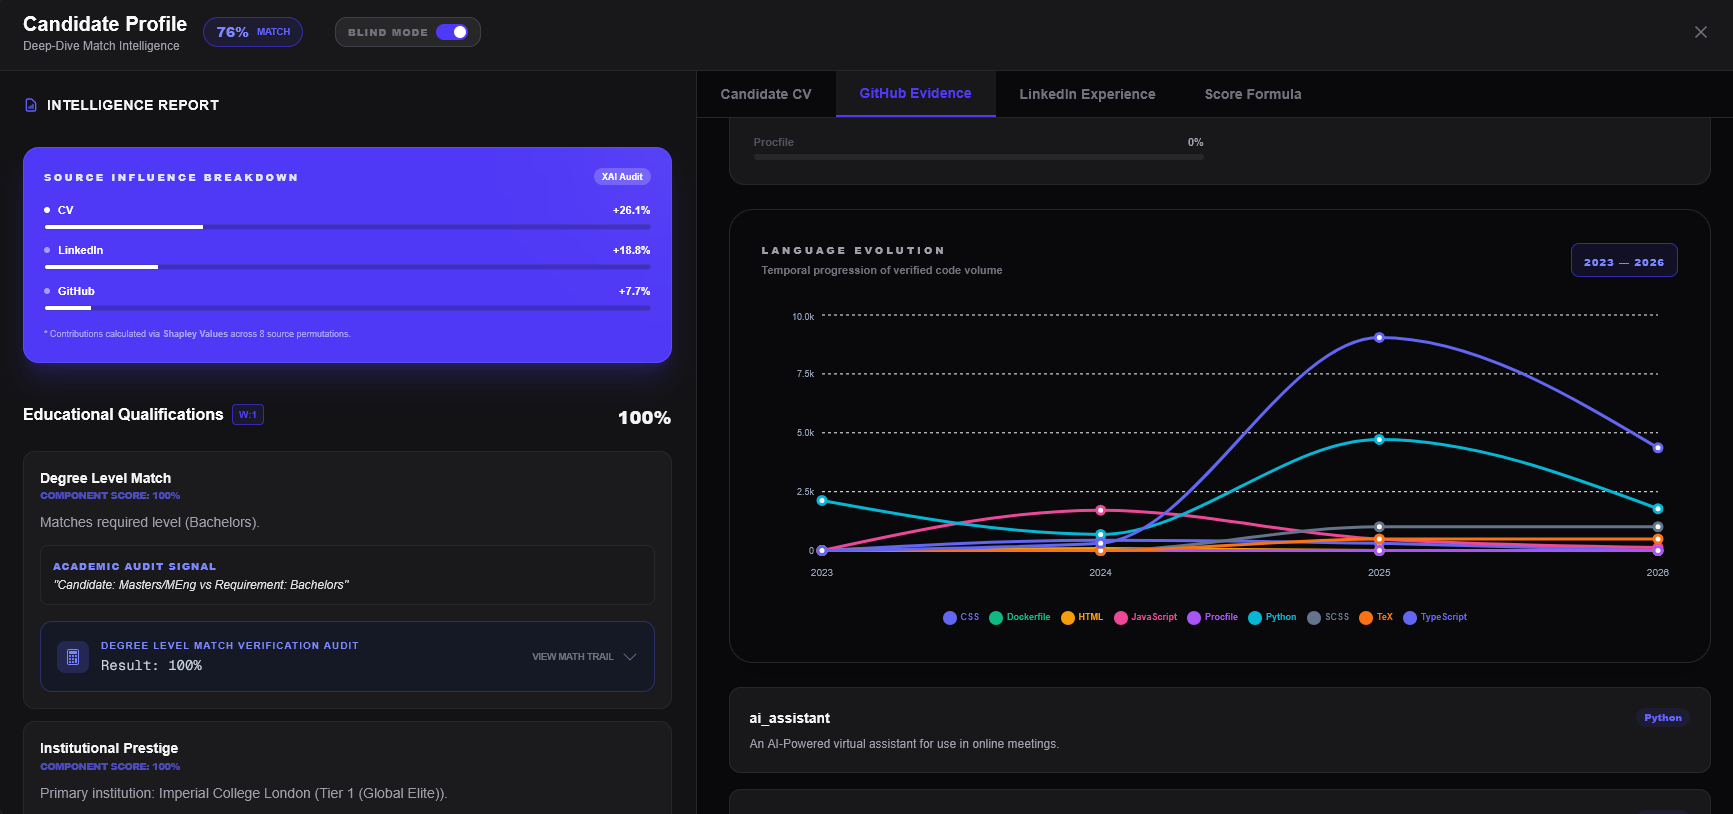
\includegraphics[width=0.95\textwidth]{implementation/screenshots/shapley_source_breakdown.png}
    \caption[Source Influence Breakdown panel]{Source influence breakdown with Shapley values per data source. In this figure,
    we show Shapley breakdown for the final match score. Shapley values for a specific metric can be viewed by clicking the ``View Math Trail''
    button}
    \label{fig:shapley_attribution}
\end{figure}


\subsection{Algorithmic Contestability}
MERIT also follows the principle of algorithmic contestability to further combat the black-box nature of these platforms.
We provide the specific evidence signals that were used to derive the score, this means that the full mathematical 
trail is provided to the recruiter to ensure that they can understand the reasoning behind the score. This in-depth
transparency is a focus of MERIT to allow recruiters to identify and override any algorithmic edge cases, or perhaps
see why a candidate got a penalisation, rather than letting this penalty go unnoticed. We ensure that the final decision
remains auditable, and aim to mitigate algorithmic bias.

The previous stage of MERIT (the execution phase) constructs both a \texttt{calculation\_summary} as well as a \texttt{results\_payload}.
For each metric, we provide the full breakdown, explicitly documenting every calculation that was performed to derive the score,
along with brief explanations for each step. Please refer to Appendix \ref{appendix:math_trail} 
for a complete step-by-step visualisation of the audit trail of an extensible metric.

This ``Glass-Box'' approach attempts to bridge the gap between complex probabilistic mathematics and practical recruitment
workflows, transforming a binary hiring decision into a defensible and interrogable process.


\subsection{Relative Cohort Normalisation}
Another common flaw with algorithmic scoring is the absence of relative context. A candidate with a year of experience may seem
weak on paper, but would be considered exceptional if the majority of the applicant pool had little to no experience. However, due
to this, the candidate would likely be undervalued if the system does not correctly highlight the difference in experience between
the candidate and the rest of the pool. To address this, MERIT also implements a dynamic cohort normalisation mechanism for the majority of
baseline metrics.

In order to achieve dynamic cohort normalisation, MERIT undergoes a two-pass approach. During the first pass of this stage, the backend
calculates the raw, absolute metrics for every candidate in the batch (such as Years of Experience, or Total GitHub repositories). Then
we aggregate these results to identify cohort maximums. In the second pass, we rerun the scoring engine, normalising candidate metrics against
the batch maximums. This approach, while not runtime efficient for extremely large datasets, ensures that MERIT's rankings remain adaptive
to the competitive landscape, rather than an arbitrary baseline.

\subsection{Glass-Box Dashboard}
\label{subsec:glass-box-dashboard}
Understandably, presenting the raw JSON \textit{results\_payload} is unreasonable due to it being inherently unscalable and poor UX.
We will briefly go over the main features of our Next.js frontend to create an intuitive, visual ``Glass-Box'' dashboard.

The first feature is probabilistic confidence labels, derived from the standard deviation $\sigma$ of the Beta distribution mentioned
in the previous chapter. We map $\sigma$ to a traffic-light badge system (Green for High, Amber for Medium, Red for Low),
allowing recruiters to instantly scan the reliability of a candidate's metric at a glance.
Non-critical penalties (e.g.\ keyword stuffing) show an amber icon on the ranking table, critical penalties (e.g.\ identity squatting) show a red warning. The significance of these labels is highlighted
more so when it comes to extensible metrics, where there is more uncertainty due to the ambiguity of how such metrics may be defined,
and calculated.

Another key innovation towards the UX of MERIT is the ``Insights'' panel. When viewing the ranking tables of a candidate, recruiters can open
a ``report'' for them, which will provide them with an overlay of, not only the candidate's score, but also how it was calculated. The metric's
calculation is also provided as a human-readable string, which can be used to understand the logic behind the score.
The panel links to the full audit trail (per-source signals, Bayesian fusion, and Shapley breakdown) and surfaces actionable 
guidance where scores are limited.
Figure~\ref{fig:glass-box-dashboards} shows the ranking table with confidence 
badges and the per-metric Insights overlay (full-size screenshots in Appendix~\ref{appendix:glass-box-ui}).

\begin{figure}[htbp]
    \centering
    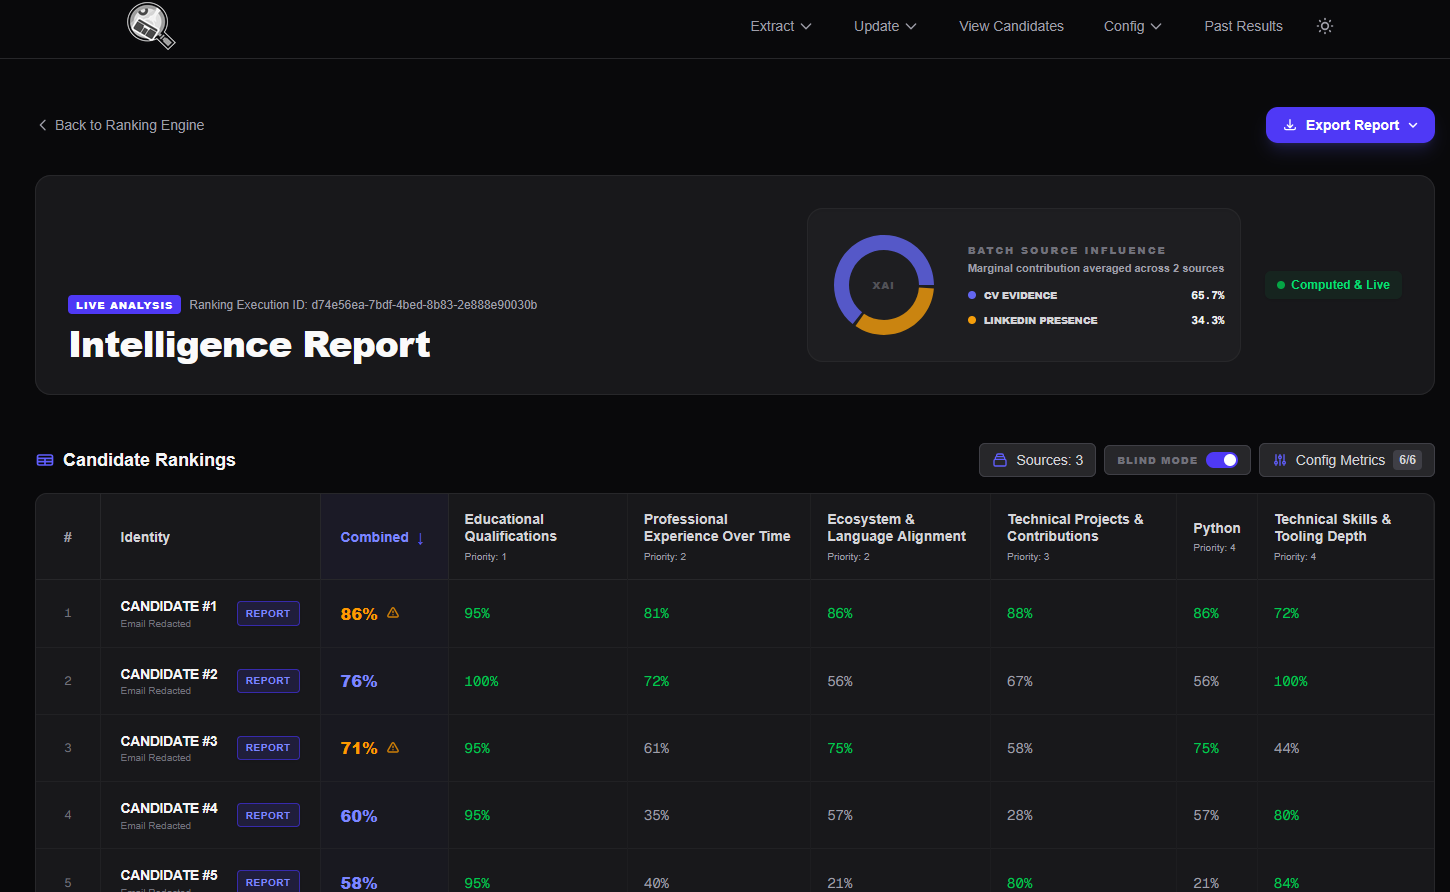
\includegraphics[height=0.17\textheight,keepaspectratio]{implementation/screenshots/candidate_rankings_dashboard.png}%
    \hfill
    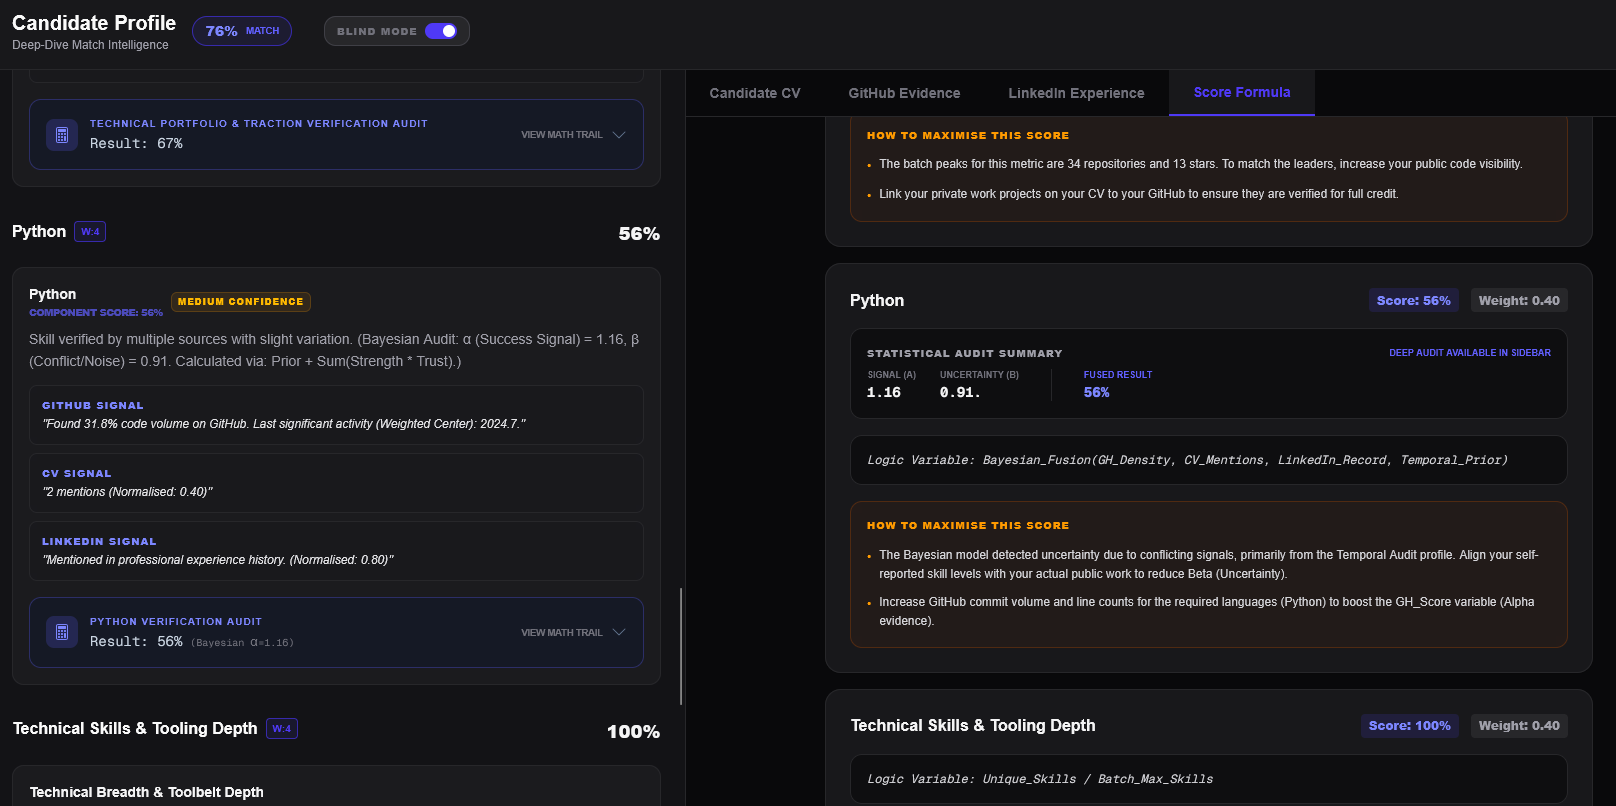
\includegraphics[height=0.17\textheight,keepaspectratio]{implementation/screenshots/metric_insights_panel.png}
    \caption[Glass-Box dashboard]{Glass-Box dashboard: Intelligence Report ranking table with confidence badges 
    (left) and Metric Insights panel for Python with audit trail (right). 
    Appendix~\ref{appendix:glass-box-ui} provides full-size versions.}
    \label{fig:glass-box-dashboards}
\end{figure}

To further aid transparency, any penalisations (such as Squatting) are also flagged to the user to highlight the negative impact of such actions on the candidate's score.
To ensure full auditability, we also provide views of each candidate's extracted data sources, so that recruiters can cross-check the audit trail.
It is also possible to view skillsets that may not have been considered by the scoring engine, for example, a configuration may have had Python
as a metric, but the candidate may have extensive work with Jupyter Notebook on their GitHub profile. If the semantic bridge mechanism fails to 
catch this, the recruiter would be able to still observe this data and potentially change their decision after accounting for this information.

\section{Bias Mitigation \& Safeguards}

TODO: Detail the cross-cutting features designed to protect the integrity of the recruitment process.

\subsection{Algorithmic Safeguards}
TODO: Implementation of the anti-keyword stuffing penalty heuristics and dynamic university tiering.

\subsection{Blind Screening Mode \& Anonymisation}
TODO: Technical implementation of redacting sensitive bias-inducing markers before UI presentation.

